The problem case laid out above is a knapsacking variation which has been shown to be NP-Hard to solve optimality.
Therefore while a solution can be found through integer programming, it is extremely slow to do and become impossible to solve for
problem cases with more than 15 jobs and 3 servers on a regular computers. \\
This means that to calculate the optimal solution, with full knowledge, then a greedy algorithm must be developed.
To do this, I have created two greedy algorithm that are compared and explained below. \\

\subsection{Greedy implementation}\label{subsec:greedy-implementation}
The first algorithm is a three stage process where the jobs are sorted on how good they are based on a metric like the
ratio of utility to resource's required. Then For each jobs in order of value, a server is selected for the jobs to run
on based on the another metric like which server has the least resources available. Resources are then allocated to a
job based on a third policy that calulcates the values for each possible allocation like the percentage of the available
resource that the allocated resources would use. The maximum of this is then chosen and allocated for the job on the server
with the process repeated till no jobs can be allocated to any server. \\
This allows for a large amount of experimentation due to the number of permutations that exists for different policies of
the different stages however any errors are propagated through the system more easily and the job value doesnt change has
the server's resources are allocated off. \\
Below is the algorithm used to generate the solution written in python with the github containing a large collection of
policies for each stage. \\

\begin{lstlisting}[language=Python]
job_values = sorted(((job, value_density.evaluate(job)) for job in jobs), key=lambda jv: jv[1], reverse=True)

# Loop through all of the job in order of values
for job, _ in job_values:
    # Allocate the server using the allocation policy function
    allocated_server = server_selection_policy.select(job, servers)

    # If an optimal server is found then calculate the resource allocation policy
    if allocated_server:
        value, (s, w, r) = resource_allocation_policy.allocate(job, allocated_server)
        job.allocate(s, w, r, allocated_server)
        allocated_server.allocate_job(s, w, r, job)
\end{lstlisting}

\subsection{Matrix Greedy implementation}\label{subsec:matrix-greedy-implementation}
The second algorithm is significantly simpler as it only uses a single policy and hopes to prevent many of the possible
problems found with the first algorithm. I believe that it will be easier to prove any approximations of the algorithm
with this version due to having a single policy compared to required three policies of the last version. \\
This algorithm works by thinking about the resource allocation first instead of last and so for each job and server
the best resource allocation is found using a metric like the product of the job utility and the percentage of the server
available resources after allocation. This is then used to generate a matrix of jobs and servers allocation with the value
being the value of the best resource allocation for the job and server pair. From this matrix then the max value is found of this
with the job then being allocated to the server and the job removed from the matrix. This is iteratively done updating each
time till all of the jobs are allocated or none of the jobs can be allocated. \\
Due to this simplification with only a single policy, I believe that this should make the algorithm better however as the
policy must include the job utility and some function of the server available resources and the resources allocation this is
less simple to find good algorithms. Therefore this is something I am still experimenting with and to prove if any
approximations are possible.

\begin{lstlisting}[language=Python]
def allocate_resources(job: Job, server: Server, value_policy: MatrixPolicy):
    # Calculates the best resource allocation by loop over all of the possible allocations that satisfy the deadline constraint
    return max(((value_policy.evaluate(job, server, s, w, r), s, w, r)
                for s in range(1, server.available_bandwidth + 1)
                for w in range(1, server.available_computation + 1)
                for r in range(1, server.available_bandwidth - s + 1)
                if job.required_storage * w * r + s * job.required_computation * r +
                s * w * job.required_results_data <= job.deadline * s * w * r), key=lambda x: x[0])


def matrix_greedy(unallocated_jobs: List[Job], servers: List[Server], value_policy: MatrixPolicy):
    while unallocated_jobs:
        value_matrix = []
        # Loop through all of the jobs and servers to calculate their best resource allocation
        for job in unallocated_jobs:
            for server in servers:
                if server.can_run(job):
                    value, s, w, r = allocate_resources(job, server, value_policy)
                    value_matrix.append((value, job, server, s, w, r))

        if value_matrix:
            # Finds the maximum value within the matrix and allocate to job and server
            value, job, server, s, w, r = max(value_matrix, key=lambda x: x[0])
            job.allocate(s, w, r, server)
            server.allocate_job(job)
            unallocated_jobs.remove(job)
        else:
            # No jobs can be allocated to servers so stop
            break
\end{lstlisting}

\subsection{Approximation}\label{subsec:approximation}
Both of these greedy algorithm are near optimal approximation algorithm with a lower bound of at least n/m of the
optimal solution. This is because at least a single job can be allocated to each server.

\subsection{Greedy algorithms results}\label{subsec:greedy-algorithms-results}
\begin{figure}
\centering
    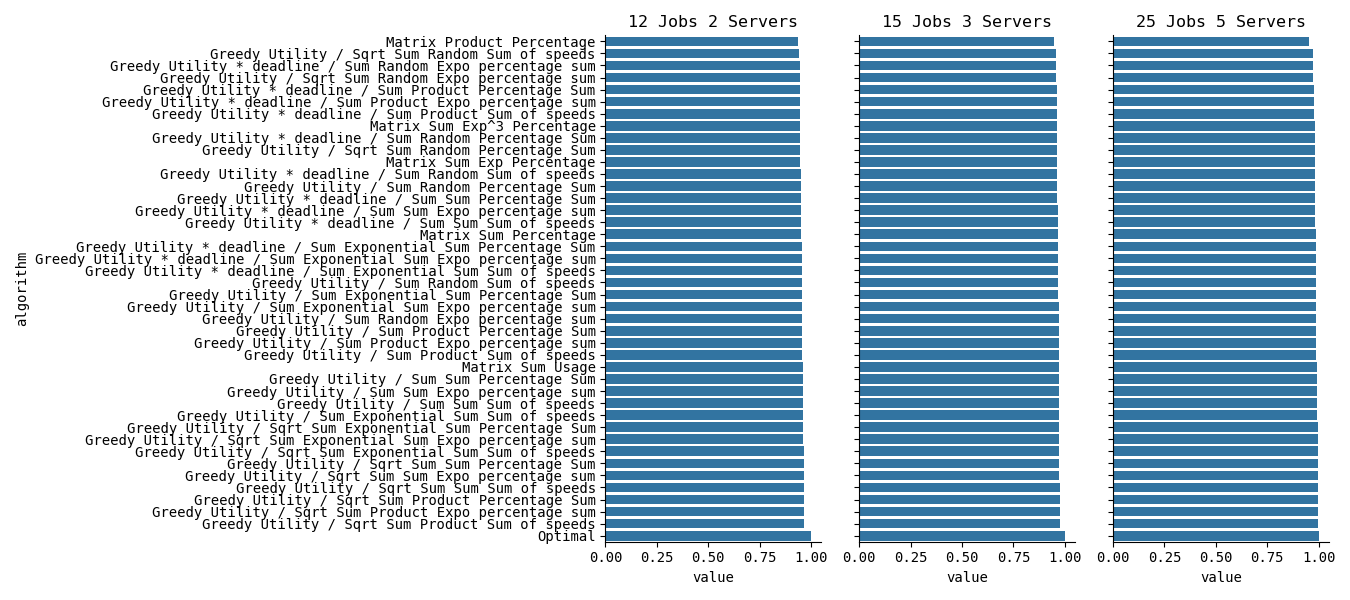
\includegraphics[width=1\linewidth]{/images/optimal_greedy_results.png}
\end{figure}
